% !Mode:: "TeX:UTF-8"
% !TEX program  = xelatex
% \documentclass[AutoFakeBold, AutoFakeSlant]{cumcmthesis}
\documentclass[withoutpreface,bwprint,AutoFakeBold, AutoFakeSlant]{cumcmthesis}    % 去掉封面与编号页
    % !Mode:: "TeX:UTF-8"
% !TEX program  = xelatex
\title{MATLAB Programming and Application}
\author{Iydon Liang}
\date{\today}

    % !Mode:: "TeX:UTF-8"
% !TEX program = xelatex

% Symbols
\newcommand{\gbt}{\texttt{GB/T 7714-2015}}
\newcommand{\python}{\texttt{Python}}
\newcommand{\mitlicense}{\texttt{MIT}}
\newcommand{\pepeight}{\texttt{PEP 8}}
\newcommand{\unicode}[1]{\texttt{U+#1}}
\newcommand{\wordcount}{\immediate\write18{if [ ! -f wordcount ]; then ./wordcount.py > wordcount; fi}\input{wordcount}}

% Packages without parameters
\usepackage{graphicx,float,subcaption}
\usepackage{amsmath,physics}
\usepackage{ebgaramond}
% \usepackage{showkeys}

% Packages with parameters
\usepackage[section]{placeins}
\usepackage[inline]{enumitem}
\usepackage[hmargin=1in,vmargin=1in]{geometry}
\usepackage[titletoc]{appendix}
\usepackage{tcolorbox}
    \tcbuselibrary{breakable,minted}
    \newtcbinputlisting{\pythonfile}[2]{
        listing engine=minted,minted style=trac,minted language=python,
        minted options={numbers=left,breaklines},
        title=\texttt{#2},listing only,breakable,
        left=6mm,right=6mm,top=2mm,bottom=2mm,listing file={#1/#2}}
\usepackage{hyperref}
    \hypersetup{
        pdfauthor={},
        colorlinks=true,
        linkcolor=black}
\usepackage{fancyhdr}
    \pagestyle{fancy}
    \renewcommand{\headrulewidth}{0.4pt}
\usepackage{unicode-math}
    \unimathsetup{math-style=ISO, bold-style=ISO, mathrm=sym}
    \setsansfont{FiraGO}[BoldFont=* SemiBold, Numbers=Monospaced]
    \setmathfont{Fira Math Regular}
\usepackage[style=gb7714-2015]{biblatex}
    \addbibresource{ref.bib}

\begin{document}

% % !Mode:: "TeX:UTF-8"
% !TEX program  = xelatex
\title{What Angle Should We Throw a Football for Maximum Range}
\author{Iydon Liang\footnote{DataHub Organization, Southern University of Science and Technology, Shenzhen, China}}
\date{\today}
\newcommand{\qepath}{sections/quadratic_equation}


\maketitle
% !Mode:: "TeX:UTF-8"
% !TEX program  = xelatex
\begin{abstract}
    We introduce projectile motion and quadratic equation through a real world problem --- \emph{what angle should we throw a football for maximum range}, then we give a proper and accurate definition of quadratic equation, from which we derive quadratic formula for solving quadratic equations. Furthermore, we list some useful applications of the quadratic equation and implement them in \texttt{Python}.
\end{abstract}
\paragraph{Keywords:} Projectile motion; Quadratic equation; \texttt{Python} simulation.

\tableofcontents\clearpage

% !Mode:: "TeX:UTF-8"
% !TEX program  = xelatex
\section{Introduction}\label{S:introduction}
\subsection{Preliminary information}
We assume that the reader has already learned the parabola in the physics class and the rectangular coordinate system in the math class. If you do not have the required knowledge, it does not matter, you can follow the information provided in this article, learning while reading.


\subsection{Projectile Motion}
Perhaps we have been told by our parents since childhood that, 45 degrees is the ideal angle to throw a football without air resistance, to understand the reasons why 45 degrees is the best angle without air resistance, we should start with projectile motion\cite{wiki:projectile_motion}.

\begin{defnbox}{Projectile motion}
    Projectile motion is a form of motion experienced by an object or particle (a projectile) that is thrown near the Earth's surface and moves along a curved path under the action of gravity only\footnote{In particular, the effects of air resistance are assumed to be negligible.}.
\end{defnbox}

In the following article, we call the curved path a trajectory\cite{wiki:trajectory}. Through experiments or simulations, we can get the trajectories of football at different angles, as shown in Figure~\ref{F:trajectory}. From the picture we can see that, the footballs are thrown from the origin, the speed remains unchanged, while the angle has changed. Intuitively, 45 degrees is indeed the ideal angle to throw a football for maximum range, and complementary angles have the same range.

The trajectory was shown by Galileo to be a parabola, which is relevant to quadratic equation. No rush, we will learn the basics of quadratic equation, in the next section.

\begin{figure}
    \centering
    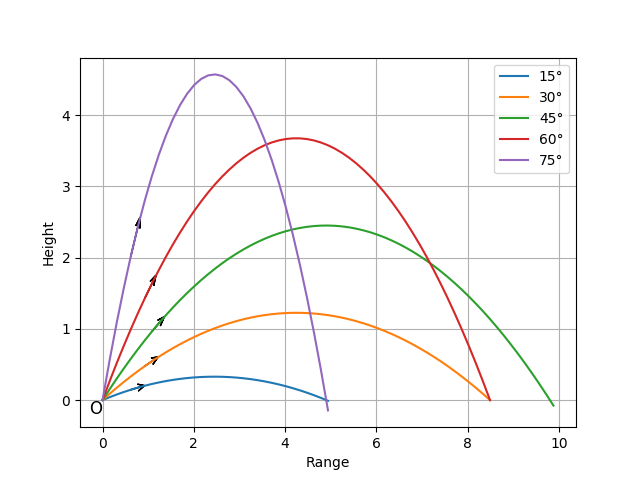
\includegraphics[width=.7\textwidth]{figures/quadratic_equation-1.png}
    \caption{Parabolic trajectories at different angles}\label{F:trajectory}
\end{figure}



\section{Quadratic Equation}\label{S:quadratic}
\subsection{Definition}
\begin{defnbox}{Quadratic equation\cite{wiki:quadratic_equation}}
    In algebra, a quadratic equation (from the Latin \emph{quadratus} for ``square'') is any equation having the form
    \begin{equation}\label{E:1}
        c_2 x^2 + c_1 x + c_0 = 0,
    \end{equation}
    where $x$ represents an unknown, and $c_n$ ($n=0,1,2$) represent known numbers, with $a\neq 0$. If $a=0$, then the equation is linear, not quadratic, as there is no $c_2 x^2$ term. Then we can divide both sides of the equation by $c_2$, and replace $c_1/c_2$ with $b$, $c_0/c_2$ with $c$.
    \begin{equation}\label{E:quadratic-equation}
        x^2 + bx + c = 0.
    \end{equation}
    That is, every quadratic equation can be transformed into the form of Equation~\eqref{E:quadratic-equation}.
\end{defnbox}


\subsection{Quadratic Formula and Its Derivation}
From Equation~\eqref{E:quadratic-equation}, we can complete the square to derive a general formula to solve quadratic equations. Then we have noticed that, coefficient of $x^2$ is 1, coefficient of $x$ is $b$, if we want to complete the square form, we have
\begin{equation}\label{E:quadratic-formula-1}
    \begin{aligned}
        x^2 + bx + c &= 0 \\
        x^2 + 2\frac{b}{2}x &= -c \\
        \left(x+\frac{b}{2}\right)^2 &= -c + \frac{b^2}{4} \\
        \left(x+\frac{b}{2}\right)^2 &= \frac{b^2-4c}{4}.
    \end{aligned}
\end{equation}

The left side of the Equation~\eqref{E:quadratic-formula-1} is a squared form, which means that it may have multiple solutions. That is, if $b^2-4c\geq 0$,
\begin{equation}\label{E:quadratic-formula-2}
    \begin{aligned}
        x + \frac{b}{2} &= \pm \frac{\sqrt{b^2-4c}}{2} \\
        x &= -\frac{b}{2} \pm \frac{\sqrt{b^2-4c}}{2} \\
        x &= \frac{-b\pm\sqrt{b^2-4c}}{2}.
    \end{aligned}
\end{equation}

If we substitute the Equation~\eqref{E:quadratic-formula-2} back to the Equation~\eqref{E:quadratic-equation}, we will find that the equation still holds. That is the quadratic formula is
\begin{equation}\label{E:quadratic-formula}
    x = \begin{cases}
        \frac{-b\pm\sqrt{b^2-4c}}{2} & \text{If $b^2-4c\geq 0$;} \\
        \frac{-b\pm i\sqrt{4c-b^2}}{2} & \text{If $b^2-4c<0$.}
    \end{cases}
\end{equation}

You can get an intuitive feel for the quadratic equation from Figure~\ref{F:quadratic-formula}. Moreover, we found other interesting phenomena --- vertex, which is the extreme point of the parabola, whether minimum or maximum. The $x$-coordinate of the vertex will be located at $x=-\tfrac{b}{2}$, and the $y$-coordinate of the vertex may be found by substituting this $x$-value into the function, which gives that $y=\tfrac{1-(b^2-4c)}{4}$.

\begin{figure}
    \centering
    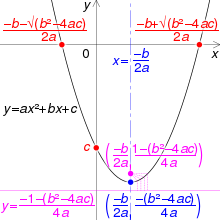
\includegraphics[width=.35\textwidth]{figures/quadratic_equation-2.png}
    \caption{Visualization of quadratic equations (with $a=1$)}\label{F:quadratic-formula}
\end{figure}

% !Mode:: "TeX:UTF-8"
% !TEX program  = xelatex
\section{Applications}\label{S:applications}
\subsection{Solution to Article Title}
From the definition of quadratic equation in Section~\ref{S:quadratic}, we can finally answer the question, \emph{what Angle Should We Throw a Football for Maximum Range?}

Firstly, we establish a rectangular coordinate system, as shown in Figure~\ref{F:parabolic-throwing}. We denote $\theta$ as shot angle, $V$ as initial velocity, $g$ as gravity, $S$ as distance, $t$ as time.

\begin{figure}
    \centering
    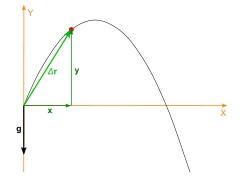
\includegraphics[width=.45\textwidth]{figures/quadratic_equation-3.png}
    \caption{Displacement and coordinates of parabolic throwing}\label{F:parabolic-throwing}
\end{figure}

Then, we have both horizontal and vertical velocity,
\begin{equation}\label{E:solution-1}
    \begin{cases}
        V_x &= V\cos(\theta) \\
        V_y &= V\sin(\theta) - gt
    \end{cases}
\end{equation}

Therefore, we have both horizontal and vertical distance at time $t$,
\begin{equation}\label{E:solution-2}
    \begin{cases}
        S_x &= V\cos(\theta)t \\
        S_y &= V\sin(\theta)t - \frac{1}{2} gt^2
    \end{cases}
\end{equation}

From Equation~\eqref{E:solution-1} and Equation~\ref{E:solution-1}, we can find all of the coordinate $(S_x, S_y)$ with angle $\theta$. From Equation~\eqref{E:solution-2}, we have $t=\tfrac{2V\sin(\theta)}{g}$, then we substitute the expression of $t$ back to the $S_y$, we have the quadratic equation
\begin{equation}\label{E:solution-3}
    S_y = \tan(\theta)S_x - \frac{g}{2V^2\cos^2(\theta)}S_x^2.
\end{equation}

From Equation~\eqref{E:quadratic-formula}, we can solve this quadratic equation, the solutions are $0$ and $\tfrac{2V^2}{g}\sin(\theta)$. Obviously, $0$ is the initial position, then the football will land at $\tfrac{2V^2}{g}\sin(\theta)$, that is, $\tfrac{V^2}{g}\sin(2\theta)$.

According to knowledge of trigonometric functions, we have the maximum range of the football is $\tfrac{V^2}{g}$, which is taken at $\theta=45$.


\subsection{Simulation of Projectile Motion}
You can use quadratic equation to simulate projectile motion, which can solve free fall problems. If you are familiar with \texttt{Python}, you can use \texttt{Python} to draw the pictures of trajectories, and you will find it easy to use Python to solve quadratic equations, especially in symbolic calculations. And the code is in Appendix~\ref{A:python}.

% !Mode:: "TeX:UTF-8"
% !TEX program  = xelatex
\section{Conclusions and Discussions}\label{S:conclusions}
From this article, we introduce projectile motion and quadratic equation through a real world problem --- \emph{what angle should we throw a football for maximum range}, then we give a proper and accurate definition of quadratic equation, from which we derive quadratic formula for solving quadratic equations. Furthermore, we list some useful applications of the quadratic equation and implement them in \texttt{Python}.
\clearpage
% !Mode:: "TeX:UTF-8"
% !TEX program  = xelatex
\section*{Acknowledgement}
The author would like to thank the Associate Editor and one referee for their valuable comments which have greatly improved the paper. The author's research is fully supported by the DataHub Organization of China (No. 1000001).
\clearpage
% !Mode:: "TeX:UTF-8"
% !TEX program  = xelatex
\nocite{rhete2008angle}
\bibliography{ref.bib}
\clearpage
% !Mode:: "TeX:UTF-8"
% !TEX program  = xelatex
\appendix
\section{Solver of LPPL in MATLAB}
\MATLAB{Title}{code/LPPL.m}


\maketitle
    % !Mode:: "TeX:UTF-8"
% !TEX program  = xelatex
\begin{abstract}
出租车已成为大多数机场乘客选择出行的主要交通工具。国内大多数机场“出发”与“到达”通道分开,出租车司机面临着 1)排队等待接客,2)直接放空返回市区 两种选择。
%为提高乘客服务效率、减少出租车运力浪费、降低司机等待成本及空载风险,设计出科学的司机载客选择方案与合理的机场周边出租车接送客调度及管制规则变得愈发重要。
本文以深圳宝安国际机场为例,从影响机场乘客与出租车司机作出双向选择的若干因素出发,构建司机决策模型;针对宝安机场外部车道构造,提出合理的乘落客区域规划方案。

针对问题一,本文从影响司机乘客双向选择的因素(乘客与司机角度)出发,运用蒙特卡罗模拟出中国45座主要城市的892条航线,估计出各机场各时间段客流量。运用多元线性回归模型,得出司机留下等待接客的概率可写为:$ P = \gamma_0 + \delta_1t + \delta_2m + \delta_3weather + \beta_1T + \beta_2S_{out} + \eta_t$。计算司机期望收益$E(\tilde{w}) = Pw_1 + (1-P)w_2$,若$E(\tilde{w})>0$,则司机应选择等待载客,且此情况下应进一步优化策略使得$E(\tilde{w})$最大;反之,司机可选择空载返回市区。

针对问题二,本文以深圳宝安国际机场为例,搜集到深圳市出租车计价规则、深圳市2016--2018年天气报告等数据,通过模拟法并验证,得到机场航班准点率及客流量,运用问题一所提出的线性模型(并推广至机器学习算法),训练模型得到最终策略。

针对问题三,本文考虑到多种国内机场的并行两车道分布实际情况(包括:机场内部电梯通道、出发入口、到达出口等各设施的具体分布),结合排队理论,综合考虑到\texttt{M/M/1},纵列\texttt{M/M/S},并列\texttt{M/M/S}三种方案,最终得出符合问题三的高效率设计方案:设置6个可同时搭载乘客的出租车候客服务台时,乘客排队等待时间成本与车道设置成本之和构成的总费用最小。

针对问题四,本文参考上海市现行机场司机多次往返载客方案,本文建议启用智能化匹配管理系统、发放电子短途票、追加日往返机场补贴三个方向,弥补出租车司机等待载客的时间成本损失,保障该类司机的“优先权”,同时建议将所需数据持久化,避免决策无数据支持。

本文编程语言为Python;深圳市天气预测数据来源为深圳市气象局官网;机场准点率信息来源为VariFlight;问题一、二中所需中国主要城市航线数模拟及各时段旅客流量由蒙特卡洛模拟及剪枝得出。


\keywords{蒙特卡洛模拟\quad 机器学习算法\quad 排队论\quad 系统最优原理\quad 边际收益递减}
\end{abstract}

    
% \tableofcontents
% \textcolor{red}{不需要目录,仅作写作参考}
% \clearpage

\section{问题重述}
    % !Mode:: "TeX:UTF-8"
% !TEX program  = xelatex
出租车已成为大多数机场乘客选择出行的主要交通工具。国内大多数机场``出发''与``到达''通道分开,送客到机场的出租车司机面临着 1)排队等待接客,2)直接放空返回市区 两种选择。

在某时间段抵达的航班数量和``蓄车池''里已有的车辆数是司机的可观测信息。通常司机可依据个人经验判断某季节或某时间段抵达航班的多少和可能乘客数量的多寡,从而决定是否在机场周边接客。机场出租车管理人员负责``分批定量''放行出租车进入``乘车区'',安排一定数量的乘客与司机双向匹配。而现实中仍有很多影响出租车司机决策的确定和不确定因素。

\begin{enumerate}[label=(\arabic*)]
    \item 分析与出租车司机决策相关因素的影响机理,即各影响因素对司机的期望收益间的数量关系,建立出租车司机选择决策模型,并给出司机的选择策略。
    \item 基于问题一所得模型,收集国内某一机场及其所在城市出租车的相关数据,给出该机场出租车司机的选择方案,并分析模型的合理性和对相关因素的依赖性。
    \item 机场落客与载客区周边常会出现出租车排队和乘客排队的情况。某机场``乘车区''现有两条并行车道,应如何设置最佳``上车点''、合理安排出租车和乘客,以保证车辆和乘客安全且使总乘车效率最高?
    \item 机场的出租车载客收益与载客的行驶里程有关,出租车司机可多次往返载客但不可拒载。管理部门拟对某些短途载客再次返回的出租车给予一定的``优先权'',使得这些出租车的收益尽量均衡(即在司机的时间成本损失上做出一定弥补),试给出一个可行的``优先''安排方案。
\end{enumerate}

    
\section{模型假设}
    \subsection{蒙特卡洛模拟数据假设}
网络上相关数据过少导致较难通过有监督的机器学习算法进行模型的训练,于是根据中国国内的真实数据进行数据建模,最后抽离出5个变量:
\begin{enumerate}
    \item 城市机场密度(将国内城市进行梯度划分)\cite{modood2018administrative};
    \item 机场停机位数量(将国内机场进行梯度划分)\cite{Pentadiine2019机场};
    \item 飞机时速(统计结果见附录~\ref{A:python-simulink}的\texttt{settings.py}文件);
    \item 飞机客容量(由搜索引擎搜索国内各大机场使用飞机型号及搭载乘客人数统计得出);
    \item 机场跑道容量\cite{wou2018跑道容量}。
\end{enumerate}

同时根据一定的规则(见附录~\ref{A:python-simulink}的\texttt{model\_airline.py}文),规划机场之间的航线,从而得到机场的客容量,由图~\ref{fig:path-a}与图~\ref{fig:path-b},从图像上来说两者基本符合。因此进一步模拟,产生各大机场的实时数据,我们选取第一梯队城市进行绘图,其中横坐标代表一天的秒数,纵坐标标示客流量,如图~\ref{fig:航空客流量},通过与能找到的少量真实数据进行比较,数据趋势大致相同,我们假设蒙特卡洛模拟可以模拟出机场总客流量。

\begin{figure}
    \centering
    \subcaptionbox{数据建模得出机场位置及航线图\label{fig:path-a}}%
        {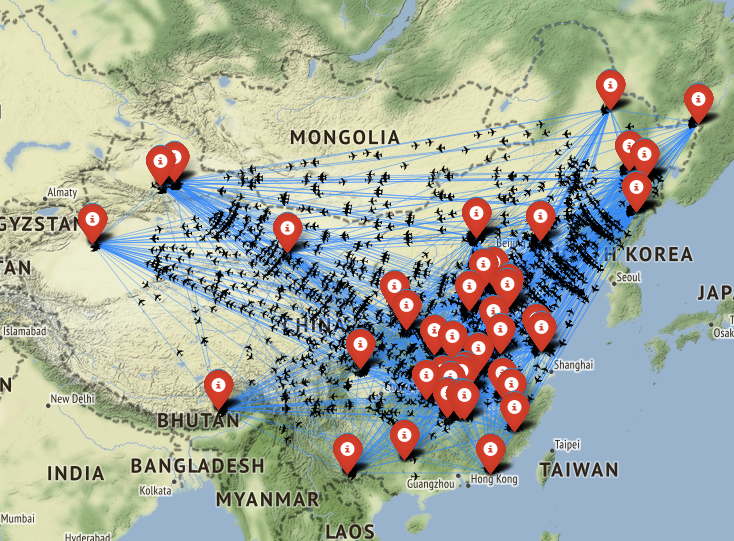
\includegraphics[width=.7\textwidth]{figures/path_python.png}} \\
    \subcaptionbox{飞常准世界航线图\label{fig:path-b}}%
        {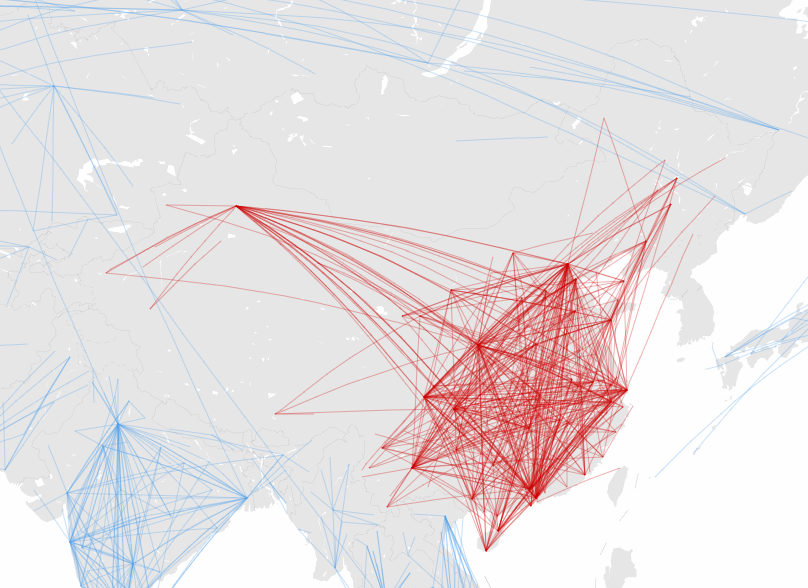
\includegraphics[width=.7\textwidth]{figures/path_variflight.png}}
    \caption{蒙特卡洛模拟与实际数据比较}\label{fig:path}
\end{figure}

\begin{figure}
    \centering
    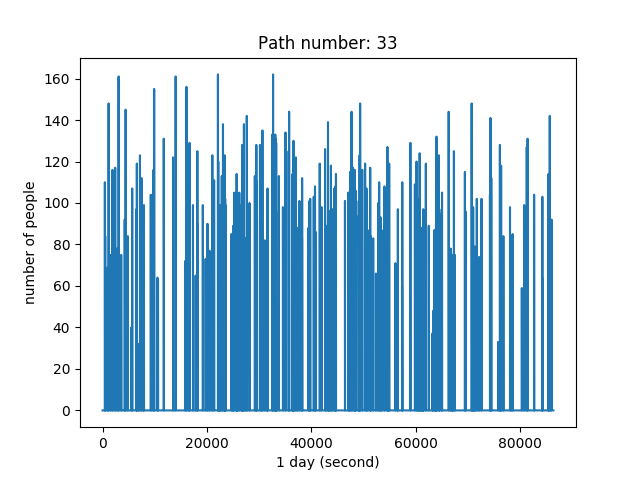
\includegraphics[width=.7\textwidth]{figures/航空客流量.png}
    \caption{实时模拟机场总客流量}\label{fig:航空客流量}
\end{figure}


\subsection{多元线性回归的五条基本假设}
\begin{enumerate}
    \item 问题一中预测司机载客概率$P$的模型可写为各解释变量的线性组合,即
        \begin{align*}
            P &= \beta_0 + \beta_1x_1 + \beta_2x_2 + \dots + \beta_kx_k + u \\
              &= \beta_0 + \sum_{i=1}^{k} \beta_ix_i + u.
        \end{align*}
        其中,$x_i (i=1,2,\ldots,k)$在本文中为各个解释变量,$k=6$,$\beta_i(i=1,2,\ldots,k)$在本文中为模型中各解释变量的系数,$u$为残差项;

    \item 假设模型含有$n$个观测值,则对于每一个观测值中的$k$个解释变量,均有且仅有一个对应的观测值;

    \item 假设各解释变量之间不相关,无完全共线性;

    \item 假设残差项关于所有解释变量的条件期望为0,即
        \[
            E(u|x_1,x_2,\ldots,x_k) = 0.
        \]

     \item 各解释变量满足同方差性,即
        \[
            Var(u|x_1,x_2,\dots,x_k) = \sigma^2,
        \]
        其中,$\sigma$是常数。
\end{enumerate}


\subsection{解释变量分布假设}
\begin{enumerate}
    \item 假设天气状态/航班延误状态服从两点分布,即
        \[
         Weather = 
         \begin{cases}
                1 & \text{航班延误/恶劣或极端天气} \\
                0 & \text{航班正常/天气晴好}
         \end{cases}
        \]
    
    \item 假设机场距乘客目的地距离$S_{out}$服从正态分布$N(10,3)$,单位为 \si{\kilo\metre}。
\end{enumerate}

    
\section{符号说明}
    \subsection{符号说明}
符号说明如表~\ref{T:symbols}。
\begin{table}
    \centering
    \begin{tabular}{@{}cc@{}}
    \toprule
    符号          & 含义              \\ \midrule
    \rowcolor[HTML]{EFEFEF} 
    $N$         & 机场乘客到达数         \\
    $N_p$       & 到达旅客中意愿乘出租车的人数  \\
    \rowcolor[HTML]{EFEFEF} 
    $m$         & 乘客行李重量          \\
    $weather$    & 天气状态,二元变量            \\
    \rowcolor[HTML]{EFEFEF} 
    $S_{out}$   & 机场距乘客目的地距离      \\
    $t_{d}$     & 司机排队等待时长        \\
    \rowcolor[HTML]{EFEFEF} 
    $T$         & 载客高峰每单平均运营时长    \\
    $P$         & 司机选择载客的概率       \\
    \rowcolor[HTML]{EFEFEF} 
    $t$         & 乘客到达时间段(乘客打车时段) \\
    $\tilde{w}$ & 司机收益(随机变量)      \\ \bottomrule
    \end{tabular}
    \caption{符号说明}\label{T:symbols}
\end{table}

    
\section{问题一的模型建立与求解}
    \subsection{问题一原理}
\subsubsection{蒙特卡洛模拟方法}
\begin{defnbox}{蒙特卡洛模拟\cite{Weisstein2019monte}}{monte-carlo}
    通过生成合适的随机数并且观察符合某些属性来解决问题的方法称为蒙特卡洛模拟(或蒙特卡洛方法、随机抽样、统计试验方法)。
\end{defnbox}

网络上相关数据过少导致较难通过有监督的机器学习算法进行模型的训练,于是根据中国国内的真实数据进行数据建模,最后抽离出5个变量:城市机场密度、机场停机位数量、飞机时速、飞机客容量以及机场跑道容量。同时根据一定的规则(见附录~\ref{A:python-simulink}的\texttt{model\_airline.py}文),规划机场之间的航线,从而得到机场的客容量。根据实际情况进行建模,使用如图~\ref{fig:architecture}所视架构,共模拟中国45座城市、892条航线、14422架飞机,为解题提供充分的训练数据。

其中程序接口易用可拓展,整体架构清晰科学,并且数据格式统一,适合用来进行机器学习算法的训练。

\begin{figure}
    \centering
    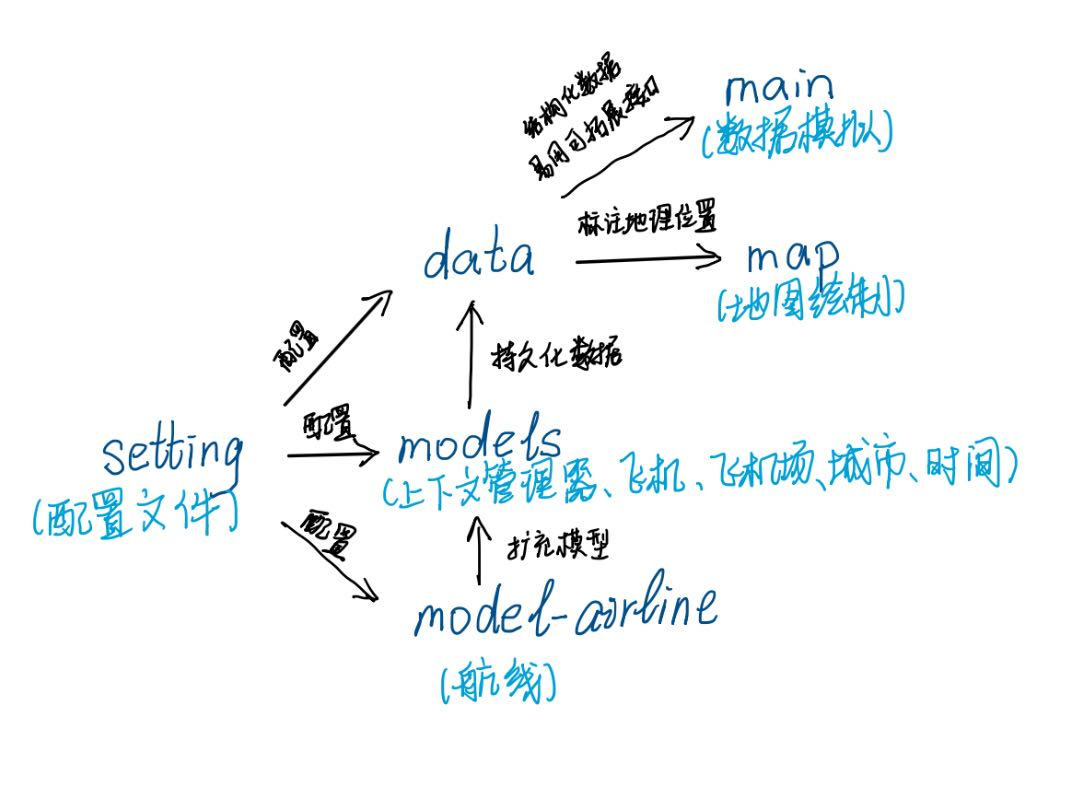
\includegraphics[width=.8\textwidth]{figures/程序架构.jpeg}
    \caption{程序架构}\label{fig:architecture}
\end{figure}


\subsection{问题一分析}
问题一旨在找出影响司机是否在机场选择载客的因素,即研究各因素与司机选择在机场载客返回市区的概率$P$的数量关系。

本文将影响因素拆分为乘客方面与司机方面两个角度。

\begin{enumerate}[label=(\arabic*)]
    \item 乘客方面,即潜在影响乘客选择出租车作为交通方式的因素分为三类:乘客到达时间段(即:乘客打车时段)$t$,乘客携带行李重量$m$,当时天气状况(即航班到达状态:延误/按时抵达)$weather$。由此三因素,进而影响当时乘客到达人数$N$及意愿选乘出租车的人数$N_p$。

    \item 司机方面,即影响司机选择在机场载客返回市区概率的因素为:乘客中意愿选乘出租车人数$N_p$,司机排队载客的平均等待时长$T$,司机的载客路程(即:机场至乘客目的地距离)$S_{out}$。
\end{enumerate}

同时使用中国范围内的直辖市、地级市、特别行政区、省会城市及各省其他主要知名城市的经纬度坐标,建立起``一城一港(北京机场设为两座航空港),两两相连''的飞行网络,见图~\ref{fig:path}。按照2018年旅客吞吐量,将我国机场大致分为四个梯队:

\begin{table}
    \centering
    \resizebox{\textwidth}{!}{%
        \begin{tabular}{ccccc}
            \hline
             & 第一梯队 & 第二梯队 & 第三梯队 & 第四梯队 \\ \hline
            \rowcolor[HTML]{EFEFEF}
            2018年旅客吞吐量 & >3000万 & 1000--3000万 & 200--1000万 & <200万 \\ \hline
        \end{tabular}%
    }
    \caption{中国机场分级依据}\label{T:classify_1}
\end{table}

蒙特卡罗模拟步骤具体如下:

\begin{enumerate}[label=(\arabic*)]
    \item 建立起“两两相连”的航空路线后,剔除始发机场与目的地机场间飞行时间短于30分钟的航线。
    
    如图\ref{fig:vector},$O$为始发港,设与其相关联的机场为$T_1$、$T_2$、$T_3$、$T_4$,已知四条航线距离$v_1$、$v_2$、$v_3$、$v_4$,根据余弦公式$\cos \theta_{ij} = |v_i\cdot v_j|/\left(|v_i|\cdot|v_j|\right)$, $i,j=1,\ldots,4$,可得出两两航空港地理位置间的夹角,夹角矩阵为$\Theta=\{\theta_{ij}\}_{i,j=1,\ldots,4} $运用离群值检验,得出临界夹角$\alpha$, $\ang{0.5}<\alpha<\ang{2}$,将$\theta$值小于$\alpha$的航线剔除。本图中,由于$O$港距$T_2$港过近且$\theta_{12}$较小,$v_2$航线可由$v_1$代替,故将$v_2$剔除。

\begin{figure}
    \centering
    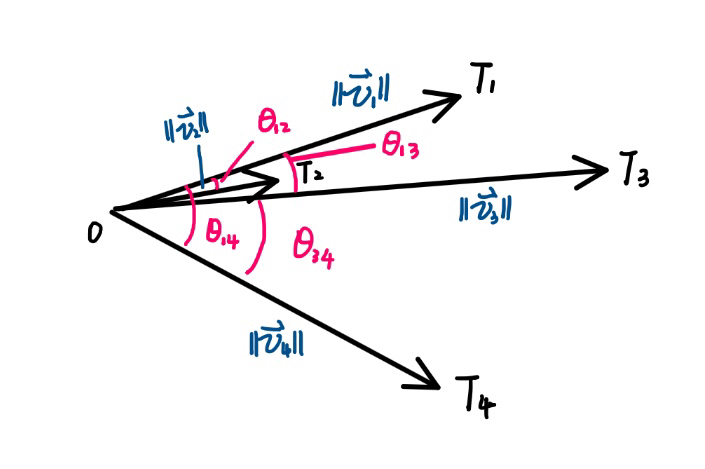
\includegraphics[width=.6\textwidth]{vector.jpg}
    \caption{飞机场节点剪枝策略}\label{fig:vector}
\end{figure}

    \item 将两地距离作为航线保留与否的权重,航线里程越长,权重越大,航线则越易被保留。计算上步剔除后各机场的节点数(即各机场的航线数),得到复杂矩阵$C_{1\times n}$,检查跨梯队间的机场是否仍存在航线联系,若存在,由于跨梯队间机场航线通常由同梯队联程航线代替,故剔除此类航线联系。
\end{enumerate}

% 航线877条
我国大陆三千万级以上机场的机位数及2018年旅客吞吐总量如表\ref{T:top10_num}所示:

\begin{table}
    \centering
    \resizebox{\textwidth}{!}{%
        \begin{tabular}{cccc}
            \hline
            IATA编号 & 机场名 & 机位数量(个) & 旅客吞吐量(万)(2018年) \\ \hline
            \rowcolor[HTML]{EFEFEF}
            XIY & 西安咸阳国际机场 & 127 & 4465 \\
            CTU & 成都双流国际机场 & 178 & 5291 \\
            \rowcolor[HTML]{EFEFEF}
            KMG & 昆明长水国际机场 & 110 & 4709 \\
            CKG & 重庆江北国际机场 & 209 & 4160 \\
            \rowcolor[HTML]{EFEFEF}
            SHA & 上海虹桥国际机场 & 155 & 4363 \\
            PVG & 上海浦东国际机场 & 218 & 7405 \\
            \rowcolor[HTML]{EFEFEF}
            CAN & 广州白云国际机场 & 220 & 6973 \\
            PEK & 北京首都国际机场 & 314 & 10098 \\
            \rowcolor[HTML]{EFEFEF}
            SZX & 深圳宝安国际机场 & 199 & 4935 \\
            HGH & 杭州萧山国际机场 & 127 & 3824 \\ \hline
        \end{tabular}%
    }
    \caption{中国大陆三千万级机场机位数及年旅客吞吐量}\label{T:top10_num}
\end{table}

 构建最直接影响$P$的因素与$P$间的数量关系,以多元线性关系为例:
 \begin{equation}\label{eq:linmodel}
    \begin{aligned}
        P &= \hat{N_p} + \beta_0 + \beta_1T + \beta_2S_{out} + \epsilon_t \\
          &= \gamma_0 + \delta_1t + \delta_2m + \delta_3weather + \beta_1T + \beta_2S_{out} + \eta_t
    \end{aligned}
\end{equation}

其中,$\beta_i$为待估计参数,$\eta_t$,$\epsilon_t$为白噪声误差项。由此,得出司机选择载客回市区的概率$P$。计算司机在此概率测度下的期望收益,即
\[
    E(\tilde{w}) = Pw_1 + (1-P)w_2,
\]
其中,$w_1$,$w_2$分别为司机载客所得收益及司机空载返回时的收益(为负)。
若$E(\tilde{w})>0$,则司机应选择等待载客,且此情况下应进一步优化策略使得$E(\tilde{w})$最大;若$E(\tilde{w})<0$,司机可选择空载返回市区。至此得到司机选择决策模型。

    
\section{问题二的模型建立与求解}
    \subsection{问题二分析}
问题二旨在将问题一得出的司机决策模型,运用到国内某一城市的机场和出租车数据上作为实证分析,并讨论模型的合理性,得出各解释变量对司机选择载客回城的概率$P$的数量关系(正/负相关及具体数值关系)。

本文选择深圳宝安国际机场及出租车数据为例,对问题一中提出的模型做检测。

% \ref{eq:linmodel}

\subsection{解释变量信息汇总}
\subsubsection{深圳出租车计价规则}
\begin{enumerate}[label=\chinese*、]
    \item ``红色''出租小汽车运价项目和标准
        \begin{enumerate}[label=(\chinese*)]
            \item 起步价:首2公里11.00元;
            \item 里程价:超过2公里部分,每公里2.40元;
            \item 返空费:每天的6时23时,超过25公里部分,每公里按上述里程价的30\%加收返空费:
            \item 夜间附加费:夜间起步价16元,每天的23时至次日凌晨6时,按上述起步价和里程价的20\%加收夜间附加费;
            \item 候时费:每分钟0.80元;
            \item 大件行李费:体积超过0.2立方米、重量超过20公斤的大件行李,每件0.50元。
        \end{enumerate}

    \item ``绿色''出租小汽车运价项目和标准
        \begin{enumerate}[label=(\chinese*)]
            \item 起步价:首1.5公里6.00元;
            \item 里程价:超过1.5公里部分,每公里2.40元;
            \item 返空费:每日6时23时,超过15公里部分,每公里按上述里程价的30\%加收返空费;
            \item 夜间附加费:每天的23时至次日凌晨6时,按上述起步价和里程价的20\%加收夜间附加费;
            \item 候时费:每分钟0.50元;
            \item 大件行李费:体积超过0.2立方米、重量超过20公斤的大件行李,每件0.50元。
        \end{enumerate}
\end{enumerate}

因``绿色''清洁能源汽车逐渐普及,故本文采用``绿色''出租车计价规则。


\subsubsection{深圳气候概况二元变量——$weather$}
下表~\ref{tab:weather_report}统计了2016-2018年深圳市极端天气日数,以此作为计算二元变量$weather$取不同状态数时的概率。

\begin{table}
    \centering
    \resizebox{\textwidth}{!}{%
        \begin{tabular}{ccccc}
            \hline
            要素 & 2018年(天) & 2017(天) & 2016年(天) & 累年平均值(天) \\ \hline
            \rowcolor[HTML]{EFEFEF}
            高温日数 & 2 & 7 & 5 & 4.3 \\
            低温日数 & 1 & 0 & 2 & 1.1 \\
            \rowcolor[HTML]{EFEFEF}
            大风日数 & 3 & 2 & 2 & 4.4 \\
            暴雨日数 & 8 & 11 & 11 & 9.2 \\
            \rowcolor[HTML]{EFEFEF}
            雾日数 & 0 & 0 & 3 & 3.3 \\
            霾日数 & 20 & 22 & 27 & 72 \\ \hline
        \end{tabular}%
    }
    \caption{2016--2018年深圳国家基本气象站天气日数}\label{tab:weather_report}
\end{table}

由此得
\[weather = 
    \begin{cases}
        1, & p = 34/365 = 0.093 \\
        0, & p = 1 - 0.093 = 0.907
    \end{cases}.
\]

\begin{figure}
    \centering
    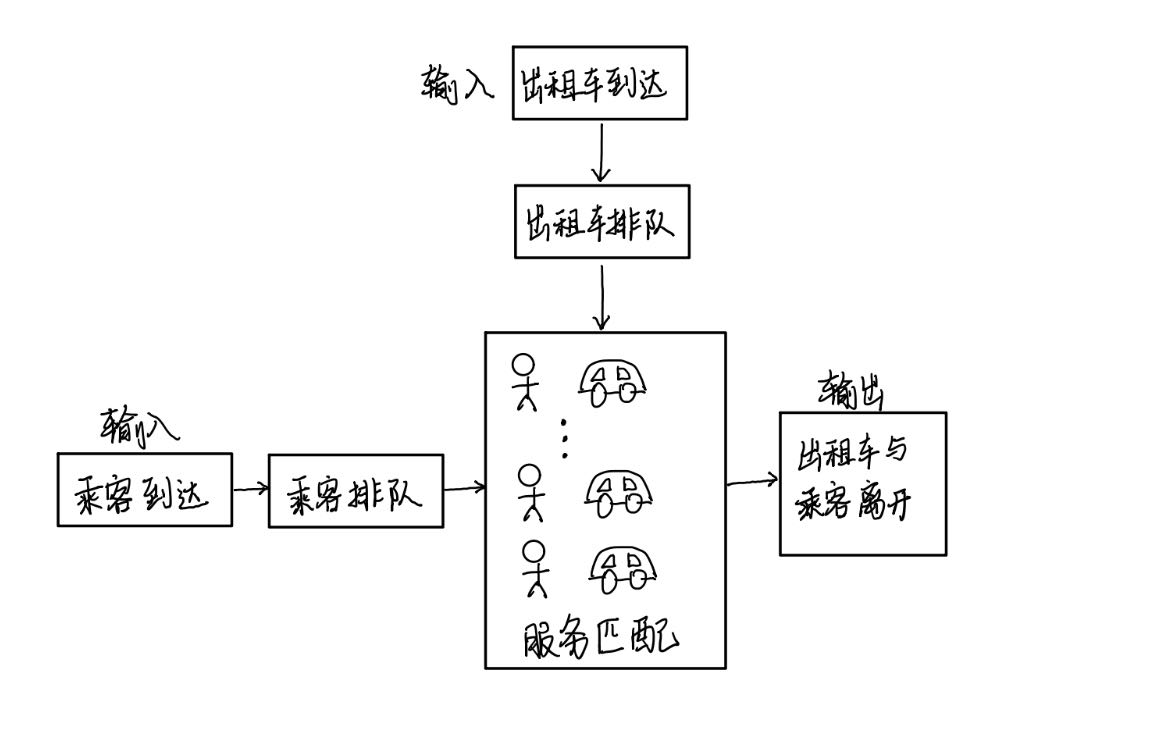
\includegraphics[width=.6\textwidth]{service.jpg}
    \caption{服务布局系统简图}\label{fig:service}
\end{figure}

\subsubsection{司机等待时长$t_d$}
假设司机等待时长服从泊松分布,即$t_{d}\~Poisson(30)$,单位为分钟。

对于排队或说等待问题来说,需考虑的因素是排队长度$L$和顾客等待时间$W$,无论是从系统的角度还是从顾客的角度来看,两者均是越小越好。对服务布局系统进行了研究,如图~\ref{fig:service}。其中队列长$L_q$是指系统中正处于排队等待的平均旅客数,队长$L_S$则是指队列长$L_q$与正在接受服务的顾客数之和。等待时间$W_q$则是指顾客从进入系统开始到开始接受服务的平均时间,逗留时间$W_s$是指从顾客进入系统到接受完服务离开系统的平均时间。

用系统中乘客排队的队长$L_s$及其逗留时间$W_s$对系统进行分析,得:
\begin{equation}\label{eq:排队系统乘客队长-1}
    L_s = L_q + C_\rho = \frac{1}{C!}\frac{(C\rho)^C\rho}{(1-\rho)^2}P_0 + \frac{\lambda}{\mu},
\end{equation}

\subsubsection{行李重量$m$}
大部分民航公司的免费托运行李额为20kg,而实际旅程中乘客携带行李重量层次不一,且尚无直接渠道得到旅客行李托运信息,因此本文认为$m$是不易观测变量,建议使用其他代理变量加入到回归式中。

$m$对民航公司是显式直接以观测变量,本文建议在实际问题解决中考虑该变量对总概率$P$的影响。

% \subsection{到达旅客中意愿乘出租车的人数$N_p$}

% \subsection{模型合理性}
% \subsection{因变量与解释变量数量关系}
%    着重看正/负相关

    
\section{问题三的模型建立与求解}
    \subsection{问题三分析}
\subsubsection{排队模型}
\begin{defnbox}{排队模型}{queue}
    排队系统主要由输入过程、排队规则和服务机构构成。输入过程,即顾客到来的时间规律,出租车辆到达的时间规律常被视为服从泊松分布;排队规则,即顾客以何种规则排队,可分为损失制、等待制、混合制;服务机构,可分为单服务台、多服务台并/串联、混合型;服务规则多样,有先到先得、后到先得、随机服务、优先服务等规则。其表示方式为:\verbbox{X/Y/Z/A/B/C}。其中,
    \begin{itemize}
        \item \verbbox{X}表示顾客到达流或顾客到达间隔时间的分布;
        \item \verbbox{Y}表示服务时间的分布;
        \item \verbbox{Z}表示服务台数目;
        \item \verbbox{A}表示系统容量限制;
        \item \verbbox{B}表示顾客源数目;
        \item \verbbox{C}表示服务规则。
    \end{itemize}
\end{defnbox}

定义$\lambda$为单位时间车辆平均到达率,$\mu$为单位时间系统服务率, 定义$\rho$为服务强度,$\rho=\lambda/\mu$。$\rho<1$, 则系统服务率大于车辆平均到达率满足服务要求,反之不能满足。

\verbbox{M/M/1}(单点式排队系统)排队模型认为车辆的到达服从泊松分布,出租车服务时间服从负指数分布,仅有一个服务台服务。布局形式如图~\ref{fig:MM1_draw}。\verbbox{M/M/S}模型则有多个服务台服务。

\begin{itemize}
    \item 单点式出租车排队服务系统是指一列乘客等候上车的队伍对应一个上车点的布局形式;
    \item 多点纵列式出租车排队服务系统属于面向乘客的带有多个服务台和一个公共队伍的排队系统;
    \item 多点并列式出租车排队服务系统与多点纵列式类似,但系统内各个上车点的布置形式呈并列式。
\end{itemize}

\subsubsection{三种常见的服务布局对比}

详见表格~\ref{tab:taxi-queue-dis-advantage}

\begin{table}
    \centering
    \resizebox{\textwidth}{!}{%
        \begin{tabular}{cccc}
            \toprule
             & 优点 & 缺点 & 适用环境 \\ \midrule
            \rowcolor[HTML]{EFEFEF}
            单点式(如图~\ref{fig:MM1_draw}) & \begin{tabular}[c]{@{}c@{}}造价低;\\ 安全,乘客与出租车\\ 同时在各自的等候空\\ 间进行排队。\end{tabular} & \begin{tabular}[c]{@{}c@{}}等候时间长,只有当\\ 一个乘客服务结束离\\ 开排队系统后,后面\\ 的乘客才能接受服务。\end{tabular} & \begin{tabular}[c]{@{}c@{}}客源较少的小型\\ 枢纽站的出租车\\ 上客区或者路侧\\ 出租车服务点。\end{tabular} \\
            多点纵列式(如图~\ref{fig:juxtaMM1}) & \begin{tabular}[c]{@{}c@{}}增加了上车服务点,\\ 提高了系统的服务效\\ 率。\end{tabular} & \begin{tabular}[c]{@{}c@{}}多个服务点的出租车\\ 同时驶离各自的上车\\ 点时,车辆之间易产\\ 生干扰与冲突。\end{tabular} & \begin{tabular}[c]{@{}c@{}}机场等枢纽的纵\\ 向距离较大的交\\ 通枢纽。\end{tabular} \\
            \rowcolor[HTML]{EFEFEF}
            多点并列式(如图~\ref{fig:juxtaMM2}) & \begin{tabular}[c]{@{}c@{}}分散客流,乘客离站\\ 效率提高。\end{tabular} & \begin{tabular}[c]{@{}c@{}}容易产生客流干扰及\\ 人车冲突。\end{tabular} & \begin{tabular}[c]{@{}c@{}}上客区纵向距离\\ 较短的传统枢纽。\end{tabular} \\ \bottomrule
        \end{tabular}%
    }\caption{不同出租车排队服务系统的优缺点}\label{tab:taxi-queue-dis-advantage}
\end{table}

\begin{figure}
    \centering
    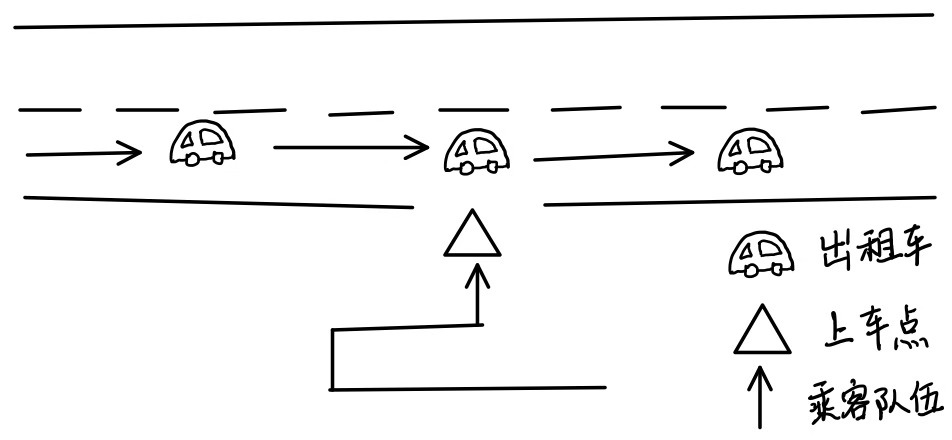
\includegraphics[width=.6\textwidth]{MM1_draw.jpg}
    \caption{\texttt{M/M/1}出租车排队服务布局}\label{fig:MM1_draw}
\end{figure}

\begin{figure}
    \centering
    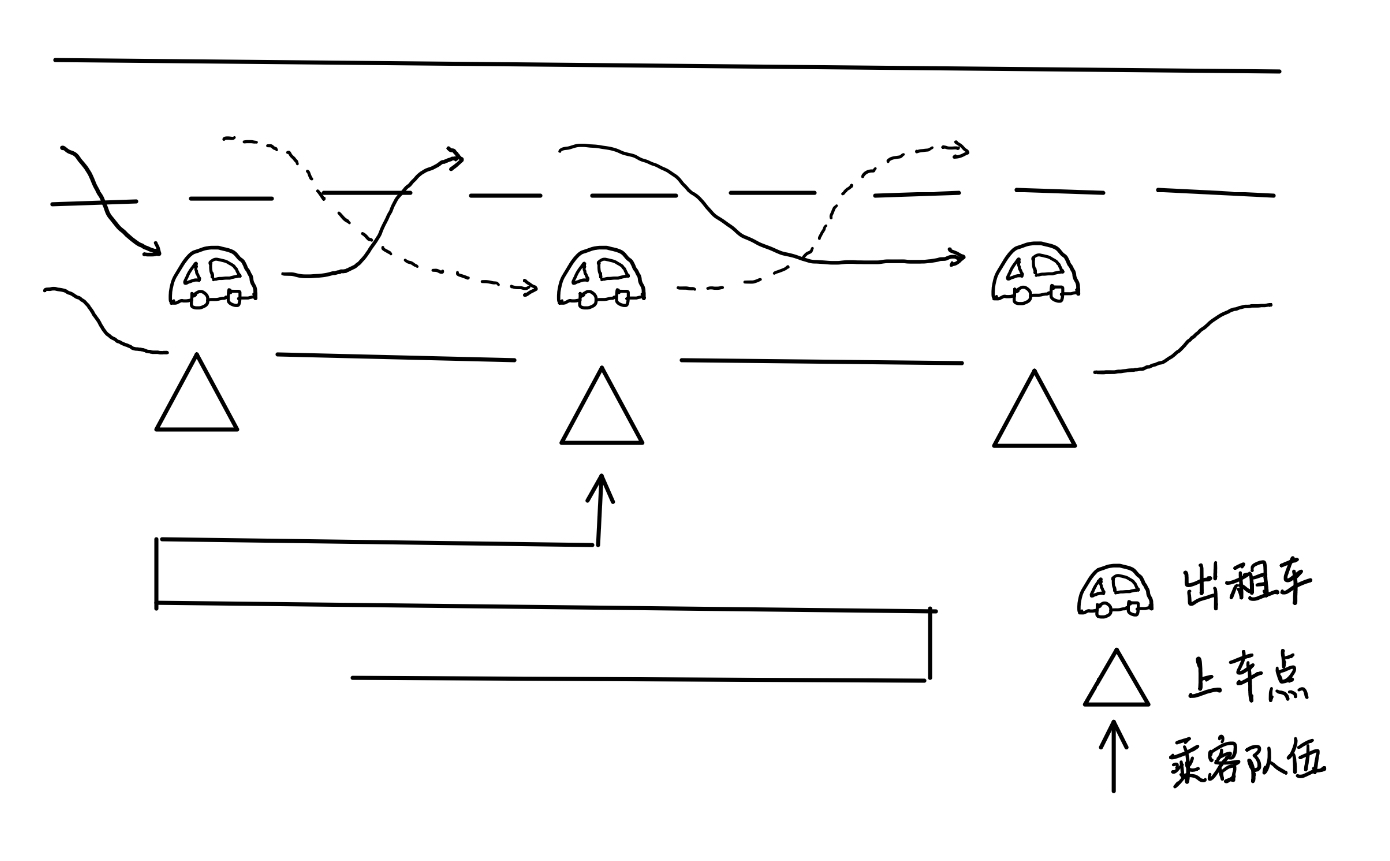
\includegraphics[width=.6\textwidth]{juxtaposeMM1.jpg}
    \caption{纵列\texttt{M/M/S}出租车排队服务布局}\label{fig:juxtaMM1}
\end{figure}

\begin{figure}
    \centering
    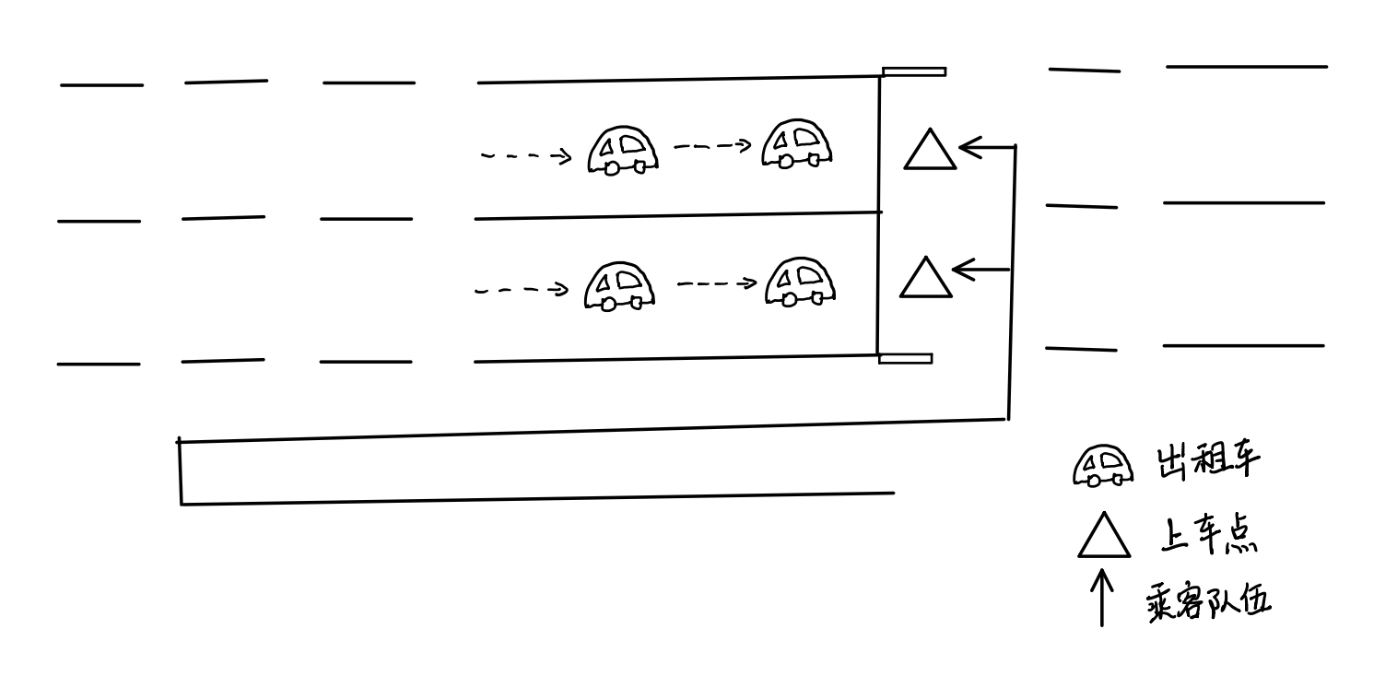
\includegraphics[width=.6\textwidth]{MM2.jpg}
    \caption{并列\texttt{M/M/S}出租车排队服务布局}\label{fig:juxtaMM2}
\end{figure}



\begin{figure}
    \centering
    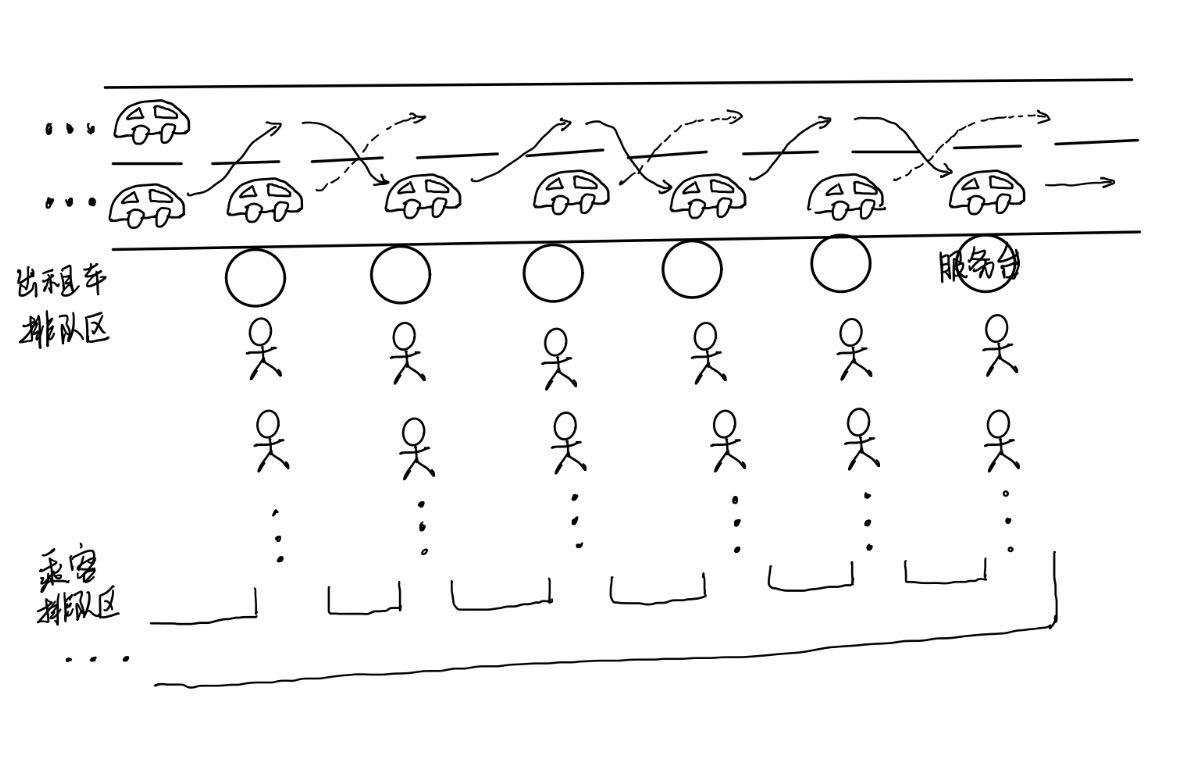
\includegraphics[width=.6\textwidth]{conclusion.jpg}
    \caption{问题三的解决方案设计简图}\label{fig:conclusion}
\end{figure}




%\begin{figure}
 %   \centering
  %  \begin{minipage}[c]{0.48\textwidth}
   %     \centering
    %    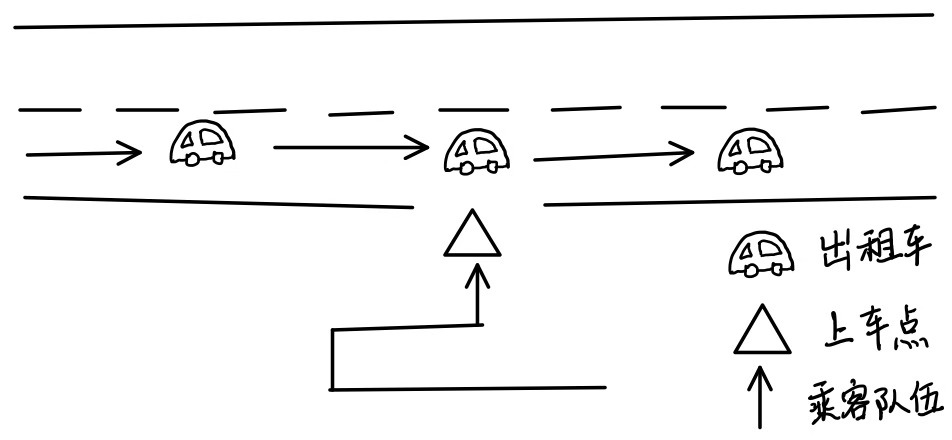
\includegraphics[height=0.2\textheight]{MM1_draw.jpg}
     %   \subcaption{M/M/1出租车排队服务布局}
    %\end{minipage}
    %\begin{minipage}[c]{0.48\textwidth}
    %    \centering
    %    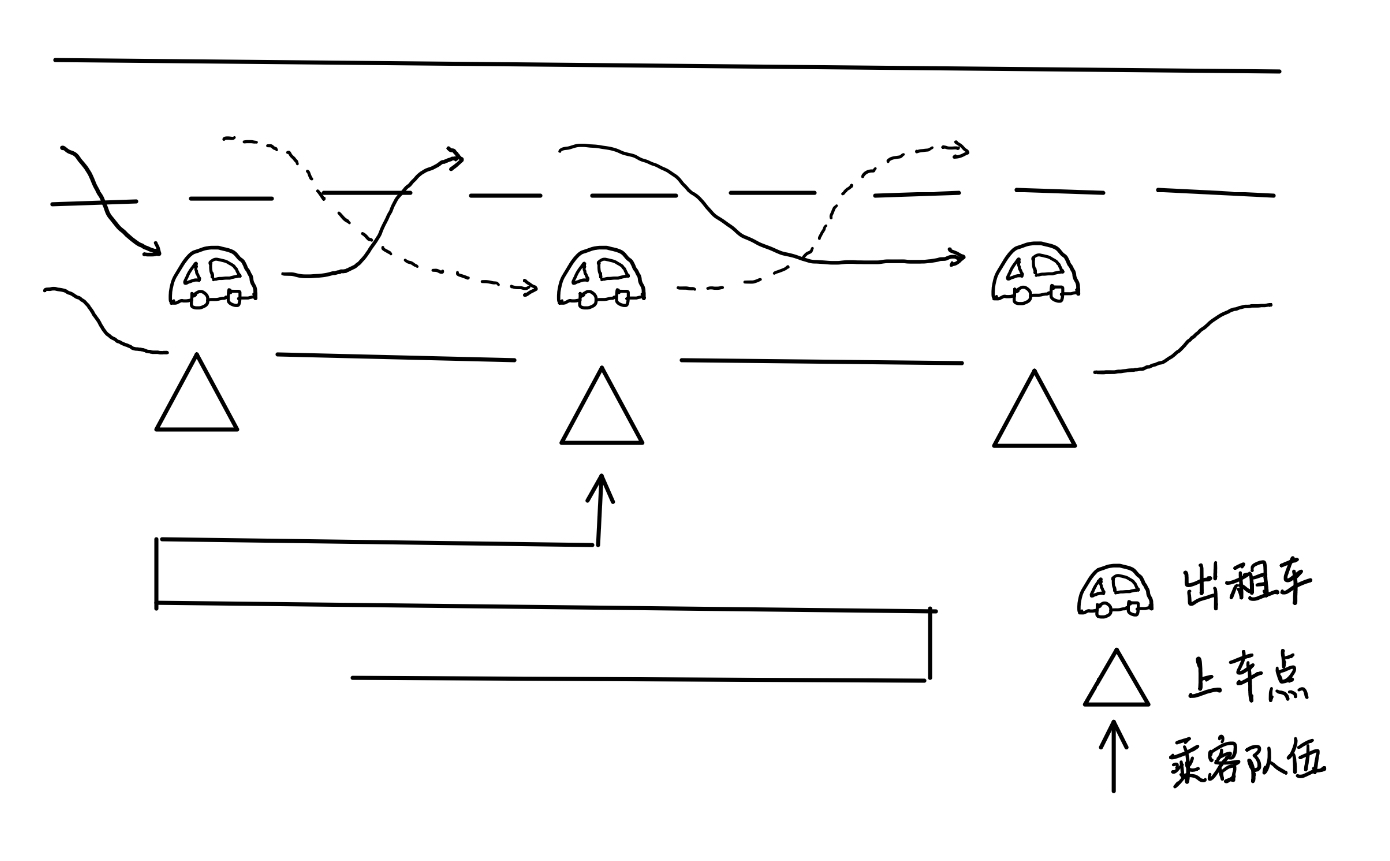
\includegraphics[height=0.2\textheight]{juxtaposeMM1.jpg}
    %    \subcaption{并列M/M/S出租车排队服务布局}
    %\end{minipage}
    %\caption{出租车排队服务系统}
%\end{figure}

\subsection{排队模型建立}
根据排队论的相关理论,对枢纽内多点式出租车上客区这一排队系统建立排队模型 。当上客区排队系 统处于全忙期,且系统的服务强度$ρ< 1$时,系统达到稳定状态且不会形成无限排队的现象,在此基础上对系统的输入与输出进行建模。

在系统达到稳态时,$C$个服务台工作,系统中出租车乘客数为$n$的概率如下:
\begin{equation}\label{eq:排队系统出租车乘客数0}
    P_0(C) = \left[\sum_{k=0}^{C-1}\frac{1}{k!}\left(\frac{\lambda}{\mu}\right)^k+ \frac{1}{C!}\frac{1}{(1-\rho)}\left(\frac{\lambda}{\mu}\right)^C\right]^{-1}
\end{equation}

\begin{equation}\label{eq:排队系统出租车乘客数n}
    P_n(C) = \begin{cases}
        \left(\lambda/\mu\right)^kP_0(C)/n, & n=1, 2, \ldots, C \\
        \left(C!C^{n-C}\right)^{-1}\left(\lambda/\mu\right)P_0(C), & n=C+1
    \end{cases}
\end{equation}

用系统中乘客排队的队长$L_s$及其逗留时间$W_s$对系统进行分析,得:
\begin{equation}\label{eq:排队系统乘客队长-2}
    L_s = L_q + C_\rho = \frac{1}{C!}\frac{(C\rho)^C\rho}{(1-\rho)^2}P_0 + \frac{\lambda}{\mu},
\end{equation}

\begin{equation}\label{eq:排队系统逗留时间}
    E(W_s) = \frac{P_n(C)}{C\mu(1-\rho)^2} = \frac{n\mu}{n!(n\mu-\lambda)^2}\left(\frac{\lambda}{\mu}\right)^nP_0(C).
\end{equation}


\subsection{排队系统优化}
利用排队系统的费用决策模型对排队系统进行优化设计。假设乘客等待时间的总费用为$Z_1=\alpha L_s$ ,上车点建设成本为$Z_2=\beta C$,其中$\alpha$为每个乘客单位时间的等待时间成本,$\beta$为单个服务台的服务时间成本与单个上车点的建设费用。当则需要满足两者之和最小才能使得系统进一步优化,即:
\begin{equation}\label{eq:最小化成本}
    \min:Z(C) = Z_1 + Z_2 = \alpha L_s(C) + \beta C, \quad Z(C-1)\leq Z(C)\leq Z(C+1)
\end{equation}

\subsection{结论}
在解决本问题时,对国内各交通枢纽已有的服务布局进行了调研,并总结出了最常见的三种进行分析讨论。并以深圳机场及题目要求为例,对多点式的排队服务系统进行了评析。利用排队论中的费用决策模型对排队系统进行优化,设计方案如图~\ref{fig:conclusion}。经过调查与计算得,当上客区的上车点数为6,即设置6个可同时搭载乘客的出租车候客服务台时,乘客排队等待时间成本与车道设置成本之和构成的总费用最小。


\section{问题四的模型建立与求解}
    \subsection{问题四分析}
问题四旨在提出对某些往返于机场短途载客的出租车司机们的``优先权''方案,本文参考上海浦东国际机场现使用的出租车智能匹配管理系统,考虑定位技术与绩效补贴两方向,同时为短途载客司机们提供``优先权''。

\subsection{大型交通枢纽出租车智能匹配管理系统}
\subsubsection{Beckmann交通分配数学模型}
交通分配模型的变量与参数表示如下:
\begin{itemize}
    \item $x_a$:路段$a$的交通流量,组成向量为$x = (\dots,x_a,\dots)$;
    
    \item $t_a$:路段$a$的交通阻抗;
    
    \item $t_a(x_a)$:以流量为自变量的阻抗函数;
    
    \item $f_k^{rs}$:点对$(r,s)$间第k条路径的交通流量;
    
    \item $C_k^{rs}$:点对$(r,s)$的第$k$条路径阻抗;
    
    \item $u_{rs}$:$(r,s)$的最小阻抗;
    
    \item $\delta_{a,k}^{rs} = \begin{cases}
            1 & \text{路段$a$在$(rs)$间的第$k$条路径}\\
            0 & \text{其他情况};
        \end{cases}$
    
    \item $W_{rs}$:$(r,s)$间的所有路径集合;
    
    \item $q_{rs}$:$(r,s)$间的交通量。
\end{itemize}

\begin{theobox}{系统最优原理}{sysOptimize}
    在交通网络中的交通量应按某种方式分配,以使网络中所有交通元的总阻抗最小。
\end{theobox}

系统最优原理的目标函数是使得网络中所有用户阻抗最小,即:
\begin{equation}\label{eq:最小用户阻抗}
    \begin{aligned}
        & \min: Z(x) = \sum_{a}x_{a}t_{a}(x_a) \\
        & \text{s.t.} \begin{cases}
            \sum_{k}f_{k}^{rs} = q_{rs} & \forall r,s; \\
            f_{k}^{rs} > 0 & \forall r,s,k; \\
            x_a = \sum_{r,s}\sum_k f_{k}^{rs}\dot\delta_{a,k}^{rs} & \forall a.
        \end{cases}
    \end{aligned}
\end{equation}
该系统称为系统最优模型(SO, System Optimization)。

\subsubsection{常见通信系统}
\begin{itemize}
    \item GSM(Global System for Mobile Communications),提供短信。
    
    \item GPRS(General Packet Radio System),介于2G与3G间的通信技术。它具有保持永远在线,按数据流量计费,自如切换、高速传输等优点。
    
    \item GPS(Global Positioning System),广泛应用、高精度。
    
    \item GIS(Geographic Information System),空间数据处理技术;与GPS、RS统称3S系统。
\end{itemize}

\subsection{短途往返出租车司机``优先权''设定}
\subsubsection{发放``智能短途票''}
传统纸质短途票发放给从机场接客且能在一个小时内或规定时间返回机场再次接客的出租车司机,以便该司机下一次返回接客时无需排队,节省等待时间成本。而纸质短途票存在票面日期被随意修改、伪造等问题,人工不易管理。

现今国内其他机场可参考上海浦东机场推行的智能化匹配管理系统,实现短途票电子到账;每部出租车均需安装GPS,以便清楚直观地看到司机是否在一定时间内``短途'',避免弄虚作假,且提高了出租车的运营效率。

\subsubsection{实行多次短途司机的奖励政策}
奖励政策具体草拟如下:

\begin{enumerate} % \begin{enumerate}
    \item 设置司机当日往返机场载客的下界次数$l$与上限$L$,上下界具体数值需依据该机场实际承载旅客量、机场周边路况等因素设置。
    
    \item 依据边际回报递减原理,令司机往返载客次数与奖金提成回报关系满足logistic函数。如图~\ref{fig:logistic}所示,$m,M$分别为奖金数的上下界,$l,L$分别为当日往返机场载客的下上限次数,点$(x_0,y_0)$为该函数段中导数最大的点。
    
    \item 导数最大即意味着边际收益最大,因此可推断出大多数司机的日往返机场载客数趋于$x_0$次,此时大部分司机的回报为$y_0$。此方案一方面能用奖金激励司机短途载客,保障了机场乘车乘客的接机需求;另一方面因接机次数存在上限及边际收益回报递减,能有效地控制司机日往返机场次数,保障了机场周边道路交通的通畅性。
\end{enumerate}

\begin{figure}
    \centering
    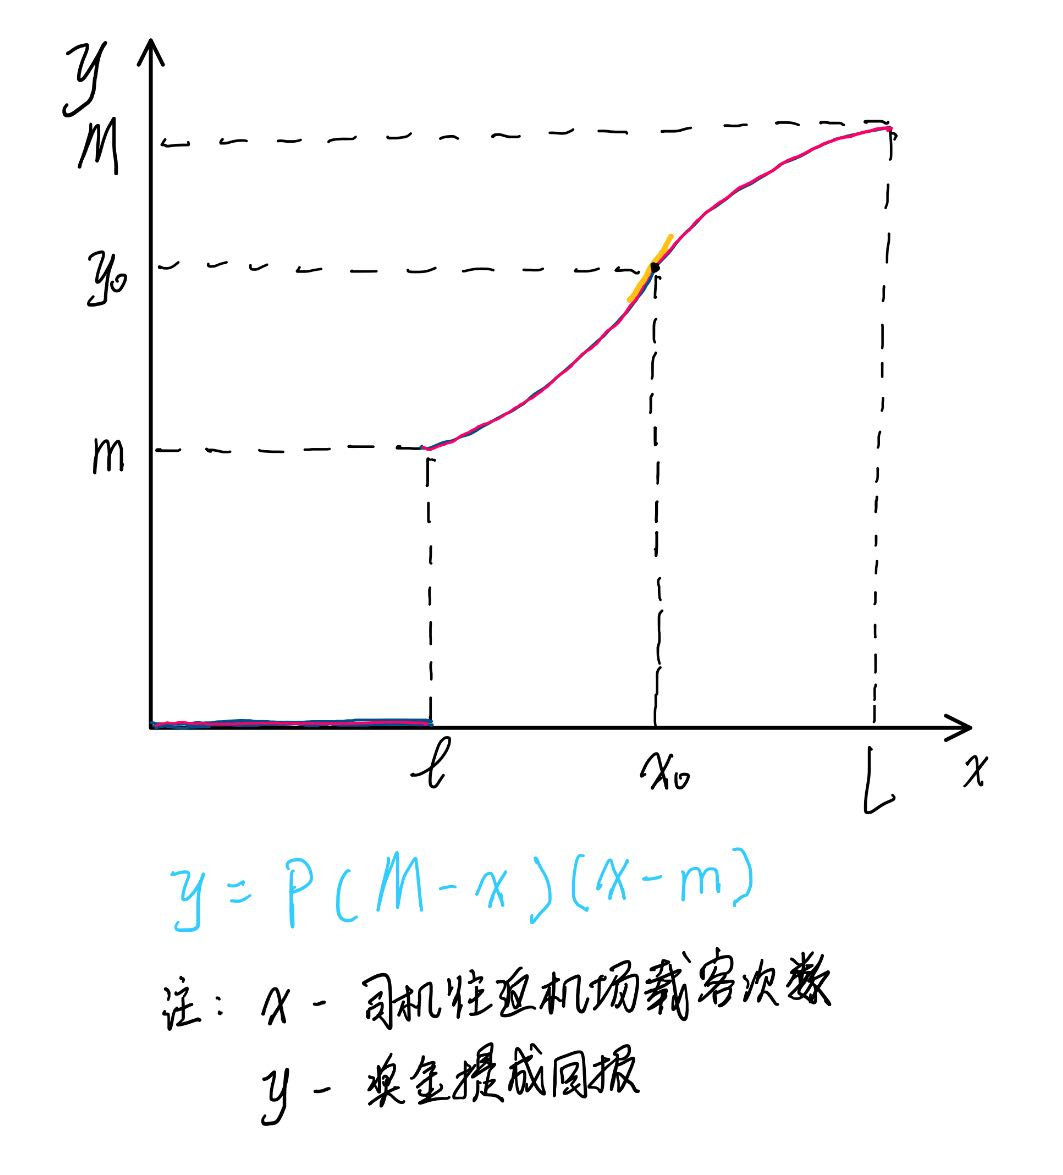
\includegraphics[width=.6\textwidth]{figures/logistic.jpg}
    \caption{司机日往返机场次数与提成回报的关系}
    \label{fig:logistic}
\end{figure}

本文建议采取电子短途票与短途接送奖励政策的同步推进,且此种方案不受机场类型、地域的影响,适宜在全国大范围推广。
    
\section{模型评价与推广}
    优点:

在问题一中,我们从出租车司机的角度出发,运用线性模型,同时兼顾到了出租车司机的利益与机场客流的疏通能力。基于蒙特卡罗模拟,综合天气等因素,较为完善地对机场乘客的数量变化规律进行了预测。

在问题二中,我们利用了深圳机场及出租车的相关数据,建立了服务布局系统,且对模型的合理性及相关因素的依赖性进行了良好评估,

在问题三中,我们建立多服务台排队模型,对国内现有的服务布局系统进行了优缺点对比。同时利用排队系统的费用决策模型对排队系统进行优化设计,通过绘图方式,清晰、直观地给出了问题的解决方案。

在问题四中,我们给出的方案是具有实用性的,因为我们对国内各大型机场都进行了调研并总结他们处理该类问题的优良办法,从而给出了可直接用于现实环境下的多种方案。

缺点:

研究中将枢纽内出租车上客区的排队系统进行了简化,仅参考了上客区的乘客排队情况。而现实中,出租车排队服务系统通常存在双端排队模式。因此,希望在后续的研究中可以综合考虑多个因素,如出租车排队情况、候客出租车停车位的设置情况等。在此基础上对排队系统进行优化,进而提高出租车乘客的离站效率。


推广:

本模型虽然存在一些不足之处,但是得到的结果还是较为合理的。本模型还可以用于火车站、大型商场等区域。在指标的方面再考虑全面,得到的结果会更让人满意。本模型基于蒙特卡罗模拟,在数据库表现方面良好,之后结合大数据、互联网+等,可解决网约车匹配等多方面问题。


\clearpage

% 参考文献
    \begin{frame}[allowframebreaks,t]{References}
    \nocite{*}
    \bibliography{ref}
\end{frame}

\clearpage

\section{附录}\appendix
    % !Mode:: "TeX:UTF-8"
% !TEX program  = xelatex
\appendix
\section{Solver of LPPL in MATLAB}
\MATLAB{Title}{code/LPPL.m}


\end{document}
